\chapter{Rotación de objetos}

\lettrine[ante=\raisebox{-1.5ex}{\LARGE ---¿},lines=2,depth=0]{T}{e
  gusta?}  ---Antonia recibió a Cecilia al día siguiente con la
sonrisa de quien hace un regalo.




    \begin{lstlisting}
$fn = 200;
// piernas
translate([10,0,0])
  cylinder(h=40,r1=3,r2=6);
translate([-10,0,0])
  cylinder(h=40,r1=3,r2=6);
// torso
translate([-18,-7,40])
  cube([36,14,40]);
// brazos
translate([23,0,45])
  cylinder(h=30,r1=3,r2=5);
translate([-23,0,45])
  cylinder(h=30,r1=3,r2=5);
// hombros
translate([23,0,75])
  sphere(r=5);
translate([-23,0,75])
  sphere(r=5);
// cabeza
translate([0,0,89])
  sphere(r=10);
    \end{lstlisting}%$


    \begin{figure}[ht]
      \centering
      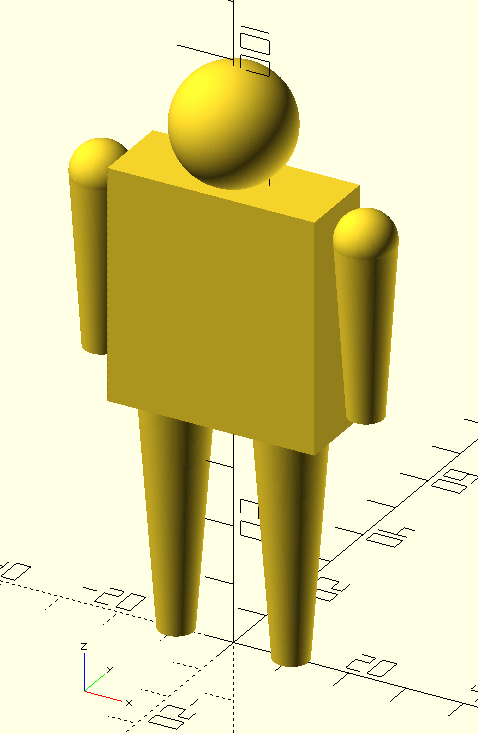
\includegraphics[width=.35\textwidth]{imagenes/robotito-1}       
      \caption{Una colección de objetos que a Cecilia se le antojó un
        robotito.}
      \label{fig:robotito-1}
    \end{figure}
    
    \section{Comentarios y variantes del cilindro}

  A Cecilia le pareció simpático: ---¿Es un robotito?  ---pre\-gun\-tó.

  ---Ponele ---concedió Antonia---. Pero además me permite mostrarte
  dos características más del lenguaje, que pueden ser de tu
  interés. Por un lado, cualquier línea que comience con dos barras
  invertidas juntas (\texttt{//}) es ignorada por \openscad; por esa
  razón, podés aprovecharla para anotar en ella comentarios: pequeñas
  aclaraciones para un eventual lector humano. Y eso ---Antonia miró
  fijamente a Cecilia--- te incluye a vos: te prometo que tras unos
  días de no convivir con tu texto vas a agradecer esas pequeñas notas
  al margen.

  \guillemotright Por otro lado ---continuó con pesado tono
  di\-dác\-ti\-co---, los cilindros admiten, al momento de ser
  creados, la declaración de dos radios: \texttt{r1} (que representa
  el de la base) y \texttt{r2} (el de la `tapa').

  ---Interesante ---acotó Cecilia, tomando a su cargo el
  te\-cla\-do---. ¿Entonces puedo crear un cono anulando el radio superior
  de un cilindro?

  \begin{figure}[ht]
  \begin{minipage}[]{.5\textwidth}
    \begin{lstlisting}
$fn = 200;

cylinder(h=50,r1=20,r2=0);
    \end{lstlisting}%$
  \end{minipage}\hfill
    \begin{minipage}[]{.4\textwidth}
      \centering
      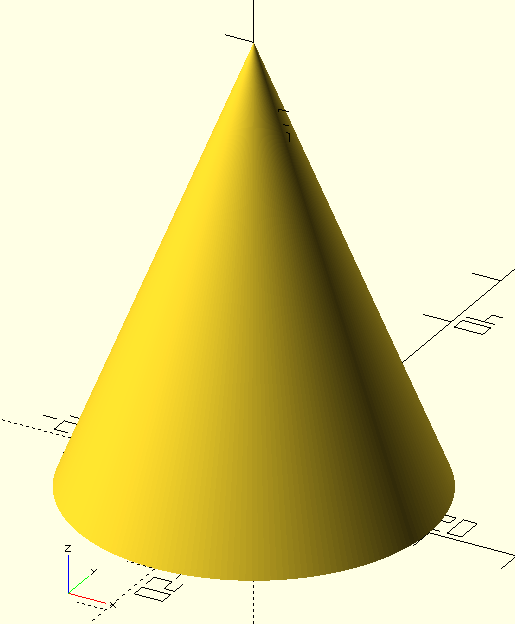
\includegraphics[width=.7\textwidth]{imagenes/cono}
    \end{minipage}
    \caption{Cecilia descubre cómo escribir un cono.}
  \label{fig:cono}
\end{figure}


---Parece que sí ---aprobó Antonia con una sonrisa de satisfacción al
comprobar que Cecilia estaba apropiándose de una de las ideas
fundamentales y más fértiles de la programación: hacerle continuamente
preguntas a la computadora bajo la forma de texto, y aprendiendo de
sus respuestas. No resultaba raro en una científica, después de todo:
ellas se dedicaban a interrogar la naturaleza con experimentos,
leyendo y desvelando sus secretos en los resultados.



  \section{Rotación}

  \guillemotright ¿No te parecería bueno que nuestro simpático robot
  fuera capaz de mover sus brazos? Para eso debemos ver cómo es
  posible rotar objetos en \openscad ---Antonia nunca fue muy hábil
  para introducir temas nuevos de manera natural---. Creo que no te
  resultará sorprendente que eso se logre con la indicación
  \lstinline!rotate!.

  \begin{figure}[ht]
  \begin{minipage}[]{.5\textwidth}
    \begin{lstlisting}
$fn = 200;

rotate([90,0,0])
  cylinder(h=30,r=5);
    \end{lstlisting}%$
  \end{minipage}\hfill
    \begin{minipage}[]{.5\textwidth}
      \centering
      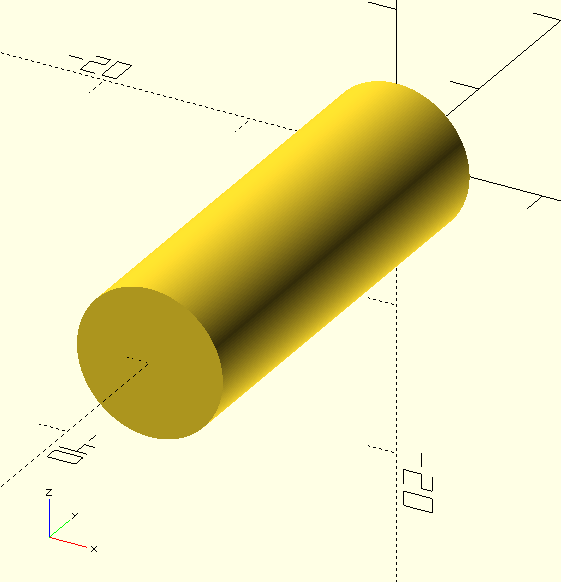
\includegraphics[width=.6\textwidth]{imagenes/cilindro-rotado-x}
    \end{minipage}
    \caption{Antonia rota un cilindro 90$^{\circ}$ alrededor del eje
      \coord{X}.}
  \label{fig:cilindro-rotado-x}
\end{figure}


\guillemotright \lstinline!rotate([x,y,z])! indica cómo debe ser
rotado el objeto al cual se aplica: `\texttt{x}' son los grados
rotados alrededor del eje homónimo, y lo mismo vale para los otros dos
ejes. En el caso del ejemplo que escribí en la figura
\ref{fig:cilindro-rotado-x}, el cilindro (originalmente creado
vertical) es rotado
90$^{\circ}$ en torno del eje \coord{X}. El ejemplo de la figura
\ref{fig:cilindro-rotado-y} hace lo propio alrededor del eje
\coord{Y}, pero usando sólo 45$^{\circ}$.

  \begin{figure}[ht]
  \begin{minipage}[]{.5\textwidth}
    \begin{lstlisting}
$fn = 200;

rotate([0,45,0])
  cylinder(h=30,r=5);
    \end{lstlisting}%$
  \end{minipage}\hfill
    \begin{minipage}[]{.5\textwidth}
      \centering
      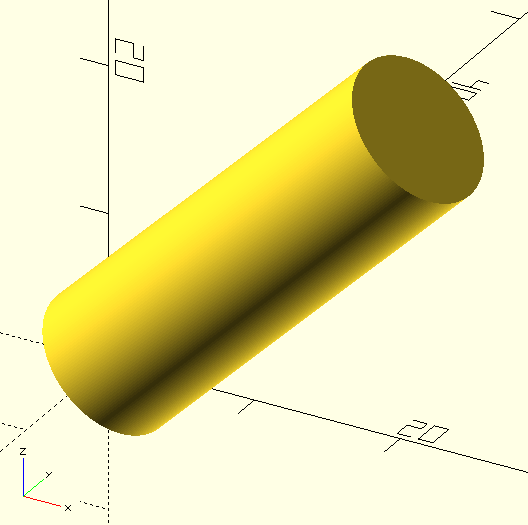
\includegraphics[width=.6\textwidth]{imagenes/cilindro-rotado-y}
    \end{minipage}
    \caption{Antonia rota otro cilindro, esta vez 45$^{\circ}$ en torno al eje
      \coord{Y}.}
  \label{fig:cilindro-rotado-y}
\end{figure}


\guillemotright Por supuesto, podés indicar más de un valor distinto
de 0 en la rotación; pero en ese caso tené en cuenta que primero se
aplica la rotación en \coord{X}, luego la rotación en \coord{Y}, y por
último la rotación en \coord{Z}. En la figura
\ref{fig:cilindro-rotado-xyz}, por ejemplo, roté el cilindro
45$^{\circ}$ alrededor del eje \coord{X}, luego
70$^{\circ}$ en torno al \coord{Y}, y finalmente
10$^{\circ}$ respecto del \coord{Z}. Hago hincapié en el orden
---Antonia sintió la necesidad de aclarar--- ya que, como bien sabés,
las rotaciones no son conmutativas.

  \begin{figure}[ht]
  \begin{minipage}[]{.5\textwidth}
    \begin{lstlisting}
$fn = 200;

rotate([45,70,10])
  cylinder(h=30,r=5);
    \end{lstlisting}%$
  \end{minipage}\hfill
    \begin{minipage}[]{.5\textwidth}
      \centering
      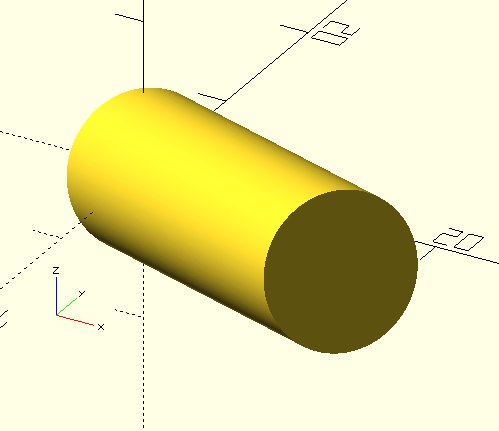
\includegraphics[width=.6\textwidth]{imagenes/cilindro-rotado-xyz}
    \end{minipage}
    \caption{Antonia aplica una rotación alrededor de los tres ejes
      coordenados a otro cilindro más.}
  \label{fig:cilindro-rotado-xyz}
\end{figure}


\section{Aplicación de varias transformaciones}


Cecilia prefirió no comentar que, efectivamente, ya lo sabía. ---¿Y
cómo hago para elegir yo misma el orden de las rotaciones?
---cuestionó, dando por descontado que era posible.

---En ese caso, y en otros similares, podés ir acumulando una
transformación detrás de otra; mejor dicho, `antes' que otra
---An\-to\-nia rió levemente de lo que sin duda consideró un
chascarrillo oportuno---. La idea es que un objeto transformado es
considerado \emph{otro} objeto en sí mismo, que puede a su vez ser
transformado, y así \emph{ad infinitum}; mirá:


  \begin{figure}[ht]
  \begin{minipage}[]{.5\textwidth}
    \begin{lstlisting}
$fn = 200;

rotate([0,10,0])
 rotate([0,0,-30])
  rotate([120,0,0])
   cylinder(h=30,r=5);
    \end{lstlisting}%$
  \end{minipage}\hfill
    \begin{minipage}[]{.5\textwidth}
      \centering
      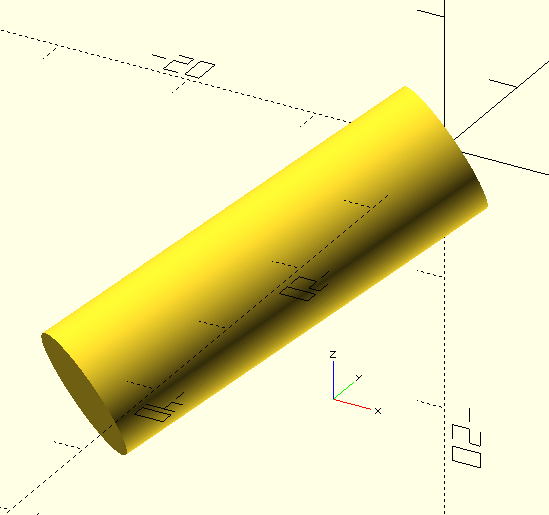
\includegraphics[width=.6\textwidth]{imagenes/cilindro-rotado-xzy}
    \end{minipage}
    \caption{Antonia aplica tres rotaciones en sucesión a... otro
      cilindro.}
  \label{fig:cilindro-rotado-xzy}
\end{figure}


\guillemotright En este párrafo ---abundó Antonia--- primero roto el
cilindro original
120$^{\circ}$ alrededor del eje \coord{X}. El resultado es un nuevo
objeto que roto
-30$^{\circ}$ en torno al \coord{Z}. Finalmente, ese nuevo objeto es
rotado 10$^{\circ}$ en el eje \coord{Y}.

  \section{Rotaciones y traslaciones}

  Cecilia no estaba segura de entender. Sintió que, para hacerlo
  plenamente, debía escribir algo que afirmara sus incipientes
  sospechas e intuiciones. Le gustó la idea de que un objeto
  transformado fuera otro objeto, susceptible de ser nuevamente
  transformado. Recordó que una traslación es una transformación.  Una
  idea destelló entonces en su mente; tomó el teclado mientras, sin
  darse cuenta, mascullaba:

  ---¿Qué pasaría si...?

    \begin{lstlisting}
$fn = 200;

// esfera de r=1
rotate([0,0,-90])
 translate([20,0,0])
   sphere(r=1);
   
// esfera de r=2
translate([20,0,0])
  rotate([0,0,-90])
    sphere(r=2);
    \end{lstlisting}%$


    \begin{figure}[ht]
      \centering
      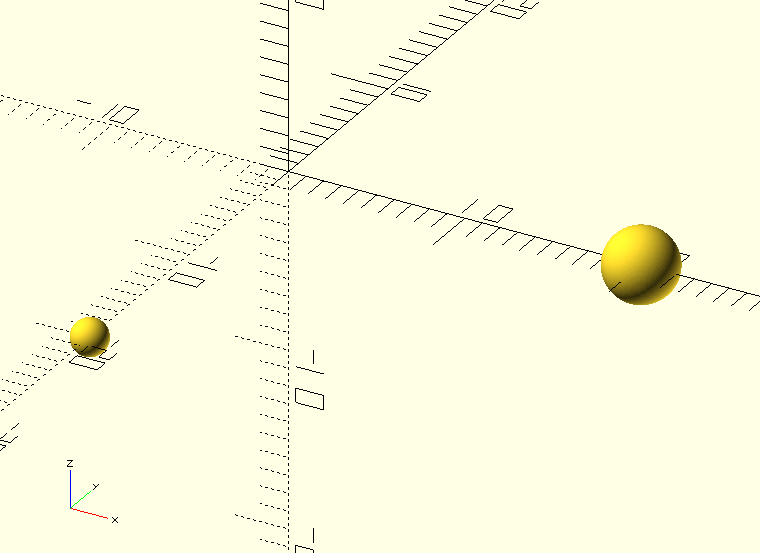
\includegraphics[width=.4\textwidth]{imagenes/esferas-rotadas}      
      \caption{Cecilia explora la posibilidad de trasladar y rotar dos esferas.}
      \label{fig:esferas-rotadas}
    \end{figure}

    Cecilia contempló el resultado de su texto con atención en la
    figura \ref{fig:esferas-rotadas}. Había escrito dos esferas de
    distinto tamaño para poder distinguirlas y así facilitar la
    comparación. A ambas las afectó con las mismas transformaciones
    (una rotación alrededor del eje \coord{Z} y una traslación a lo
    largo del eje \coord{X}); lo que cambió es el orden: la esfera de
    radio igual a 1 primero fue trasladada y luego rotada, al revés de
    lo que hizo con la segunda esfera.

  Antonia estuvo a punto de interrumpir sus pensamientos con una de
  sus explicaciones, pero Cecilia la anticipó:

  ---¡Pará!  ---dijo con tono que no admitía réplica---. Creo que ya
  lo tengo ---y volvió a sumergirse en su propio texto.

  En primer lugar, comentó casi todas las líneas del mismo, dejando
  sólo la primera esfera con la traslación. <<Buen truco>> ---pensó,
  satisfecha de su astucia---, <<así puedo concentrarme en un paso a
  la vez>>.

    \begin{lstlisting}
$fn=200;
      
// esfera de r=1
//rotate([0,0,-90])
 translate([20,0,0])
   sphere(r=1);
   
// esfera de r=2
//translate([20,0,0])
//  rotate([0,0,-90])
//    sphere(r=2);
    \end{lstlisting}%$

  
    <<Muy bien>> ---se felicitó, mientras seguía con sus
    ca\-vi\-la\-cio\-nes---; <<ahora vamos a rotar ese nuevo objeto>>.

\begin{lstlisting}
$fn=200;
      
// esfera de r=1
rotate([0,0,-90])
 translate([20,0,0])
   sphere(r=1);
   
// esfera de r=2
//translate([20,0,0])
//  rotate([0,0,-90])
//    sphere(r=2);
    \end{lstlisting}%$

    \begin{figure}[ht]
      \centering
      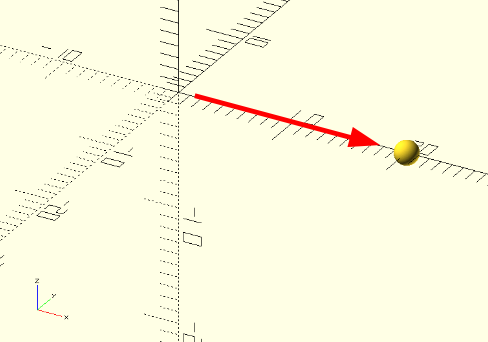
\includegraphics[width=.4\textwidth]{imagenes/esfera-trasladada}
      \hspace{.05\textwidth}
    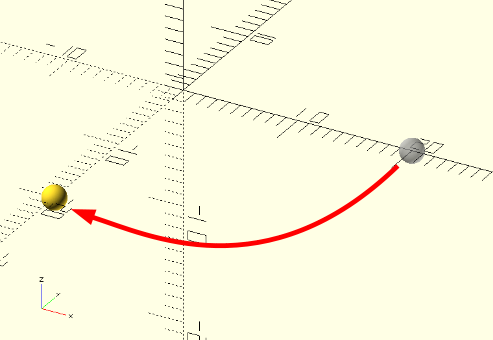
\includegraphics[width=.4\textwidth]{imagenes/esfera-trasladada-y-rotada}     
    \caption{Esfera trasladada y luego rotada.}
    \label{fig:esfera-trasladada-y-rotada}
  \end{figure}
  
    
  Cecilia pudo analizar el resultado de su texto en la imagen derecha
  de la figura \ref{fig:esfera-trasladada-y-rotada}.  <<Así que las
  rotaciones siempre refieren al origen de coordenadas: si el objeto
  está lejos de él, es rotado manteniendo su distancia respecto al
  mismo>> ---Cecilia sentía que estaba empezando a
  en\-ten\-\mbox{der---.} <<Por otro lado, la esfera 2 primero fue
  rotada>>:

    \begin{lstlisting}
$fn=200;
      
// esfera de r=1
//rotate([0,0,-90])
// translate([20,0,0])
//   sphere(r=1);
   
// esfera de r=2
//translate([20,0,0])
  rotate([0,0,-90])
    sphere(r=2);
    \end{lstlisting}%$

    
    <<Lo cual, en el caso de una esfera, es ocioso>> ---Cecilia rió
    para sus adentros, divertida---. <<¡Una esfera, después de todo,
    tiene simetría esférica! Y si ahora la trasladamos, llegará
    sencillamente a la misma posición que hubiera alcanzado sin esa
    espuria rotación previa>>:

\begin{lstlisting}
$fn=200;
      
// esfera de r=1
//rotate([0,0,-90])
// translate([20,0,0])
//   sphere(r=1);
   
// esfera de r=2
translate([20,0,0])
  rotate([0,0,-90])
    sphere(r=2);
    \end{lstlisting}%$


    \begin{figure}[ht]
      \centering
      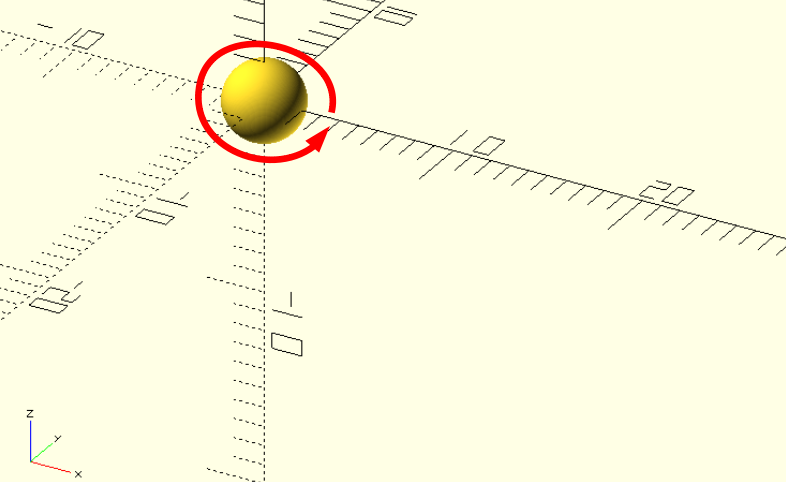
\includegraphics[width=.4\textwidth]{imagenes/esfera-rotada}
      \hspace{.05\textwidth}
      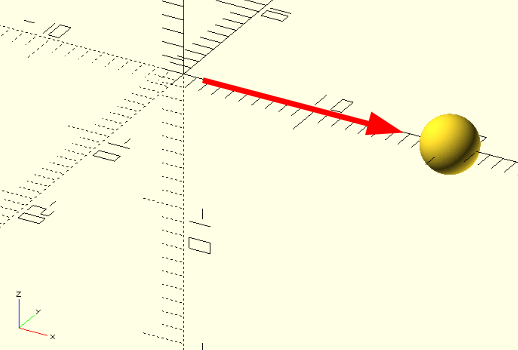
\includegraphics[width=.4\textwidth]{imagenes/esfera-rotada-y-trasladada}      
      \caption{Esfera rotada (inútilmente) y luego trasladada.}
      \label{fig:esfera-rotada-y-trasladada}
    \end{figure}
    
  \section{Rotaciones, traslaciones y bucles}

  Antonia aplaudió lentamente, con gesto de aprobación:

  ---¿Puedo decir algo ahora, o la Sra. Grace Hopper está demasiado
  enfrascada en sus grandes piezas literarias? ---di\-jo, con gesto algo
  burlón.

  Cecilia salió de su ensimismamiento algo ruborizada; sintió la
  necesidad de replicar:

  ---Cómo vos gustéis, Augusta Ada, condesa de Lovelace ---dijo,
  inclinando suave y ceremoniosamente la cabeza.

  Ambas rieron ligeramente; les gustaba intercambiarse los nombres de
  científicas célebres.  Antonia tomó el teclado y empezó a
  escribir. Mientras lo hacía, miraba a Cecilia de soslayo.

  
\begin{figure}[ht]
  \begin{minipage}[]{.5\textwidth}
    \begin{lstlisting}
$fn=200;

rotate([0,0,0])
 translate([20,0,0])
   sphere(r=2);
rotate([0,0,30])
 translate([20,0,0])
   sphere(r=2);
rotate([0,0,60])
 translate([20,0,0])
   sphere(r=2);
rotate([0,0,90])
 translate([20,0,0])
   sphere(r=2);
rotate([0,0,120])
 translate([20,0,0])
   sphere(r=2);
    \end{lstlisting}%$
  \end{minipage}\hfill
    \begin{minipage}[]{.5\textwidth}
      \centering
      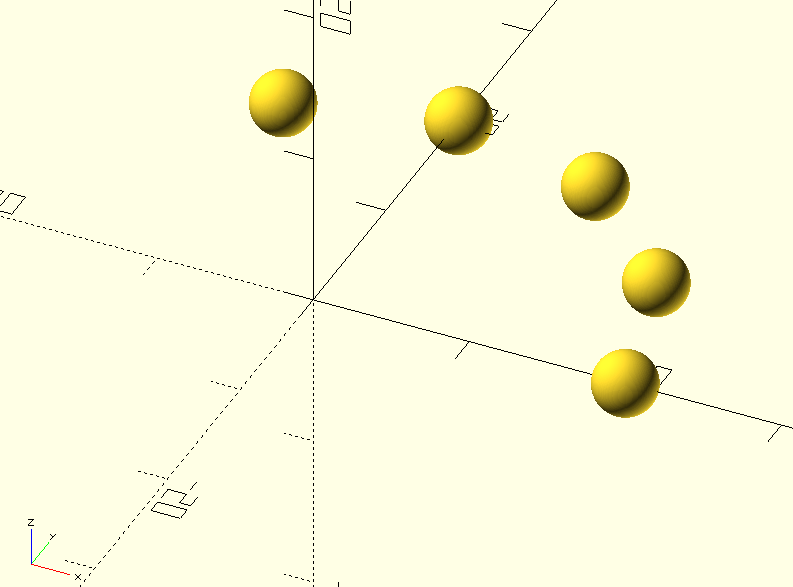
\includegraphics[width=\textwidth]{imagenes/varias-esferas}
    \end{minipage}
    \caption{Antonia escribe varias esferas esperando que una idea
      surja naturalmente en Cecilia.}
    \label{varias-esferas}
  \end{figure}
  
  Cecilia seguía con la vista las líneas de Antonia. De pronto, soltó
  en un rapto de entusiasmo:

  ---¡Pará! ¡Ya sé lo que estás haciendo! A ver, dejame a mí... ---y
  sin esperar que le respondiera, tomó el teclado para sí. Había
  notado un patrón en el nuevo texto: Antonia estaba creando esferas
  idénticas, separadas del centro de coordenadas la misma distancia y
  luego rotadas alrededor del eje \coord{Z} con ángulos múltiplos de
  15$^{\circ}$. Esa repetición regular gritaba la necesidad de un
  bucle:

\begin{lstlisting}
$fn=200;

for (alfa=[0:15:359])
 rotate([0,0,alfa])
  translate([20,0,0])
   sphere(r=2);
    \end{lstlisting}%$

    \begin{figure}[ht]
      \centering
      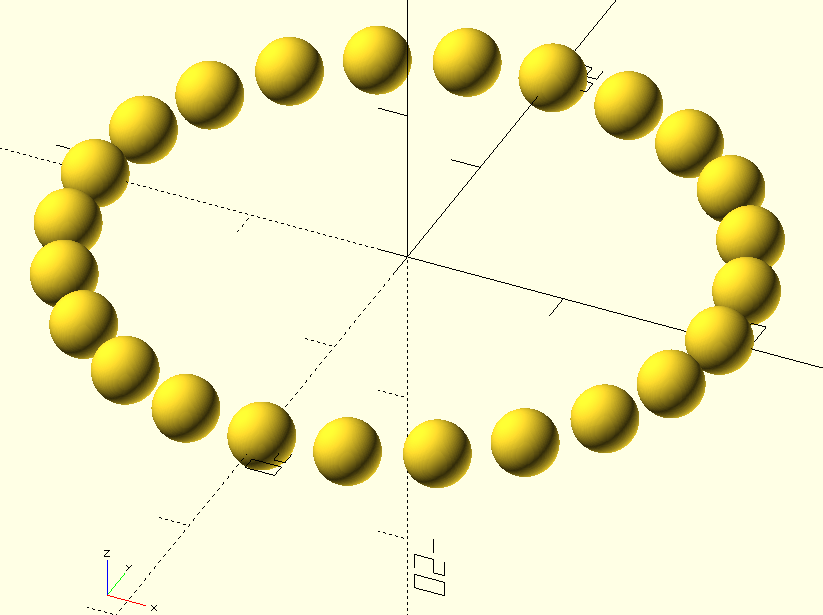
\includegraphics[width=.5\textwidth]{imagenes/anillo-de-esferas}      
      \caption{Cecilia descubre cómo escribir un anillo de esferas.}
      \label{fig:anillo-de-esferas}
    \end{figure}

    Cecilia giró su rosto en dirección a Antonia; ambas se miraron
    radiantes de alegría. Cecilia volvió a mirar el monitor; comprobó
    que su intuición funcionaba: había creado un bucle que asignaba a
    la variable \texttt{alfa} valores entre 0 y 359 en intervalos de
    15, y con ellos creaba esferas trasladadas la misma distancia y
    rotadas dicho ángulo \texttt{alfa}. Por momentos parecía demasiado
    hermoso para ser verdad.


  ---Hermoso ---Antonia confirmó sus pensamientos---.  Ahora, ¿te
  animás a hacer algo como la figura \ref{fig:anillos-de-esferas}?
  
    \begin{figure}[ht]
    \centering
    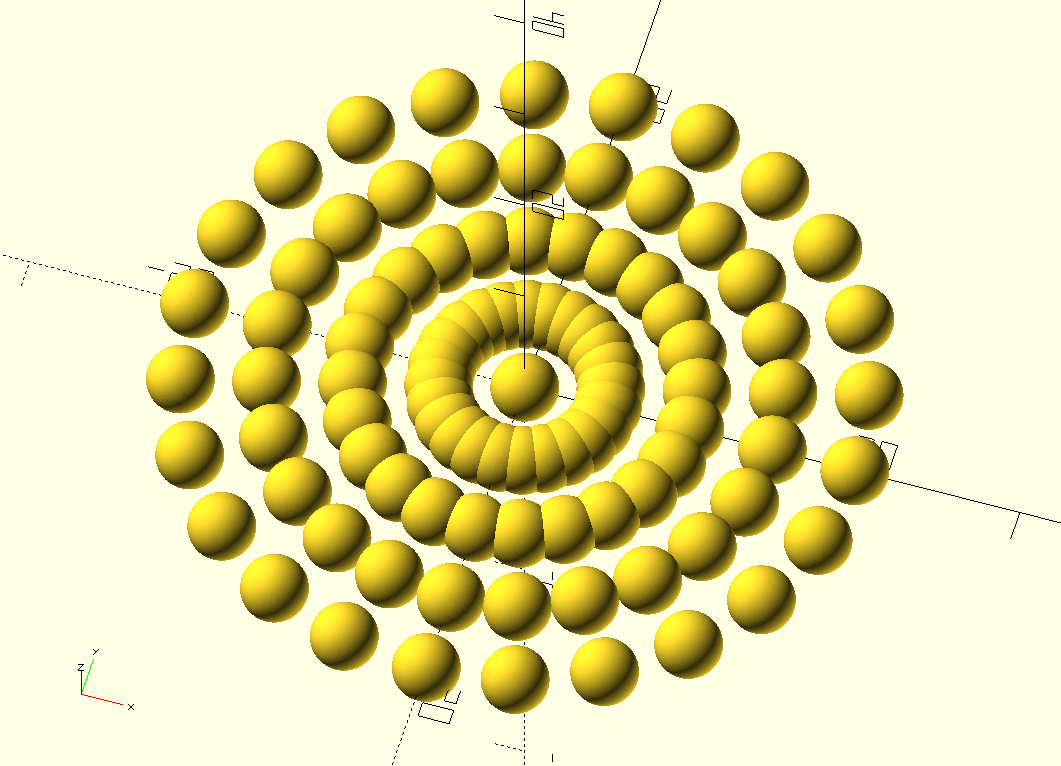
\includegraphics[width=.65\textwidth]{imagenes/anillos-de-esferas}    
    \caption{Anillos de esferas}
    \label{fig:anillos-de-esferas}
  \end{figure}



  Cecilia pegó un respingo en su silla. Trató de describir en palabras
  lo que veía. <<Parecen ser varios anillos de esferas como el mío,
  pero de radios diferentes>> ---pensó. Tras unos momentos de
  concentrada contemplación, sintió que la solución pasaba por
  utilizar otro bucle.

  \begin{figure}[b]
  \begin{minipage}[]{.5\textwidth}
    \begin{lstlisting}
$fn=200;

for(x=[20:-5:0])
 for (alfa=[0:15:359])
  rotate([0,0,alfa])
   translate([x,0,0])
    sphere(r=2);
    \end{lstlisting}%$
  \end{minipage}\hfill
    \begin{minipage}[]{.5\textwidth}
      \centering
      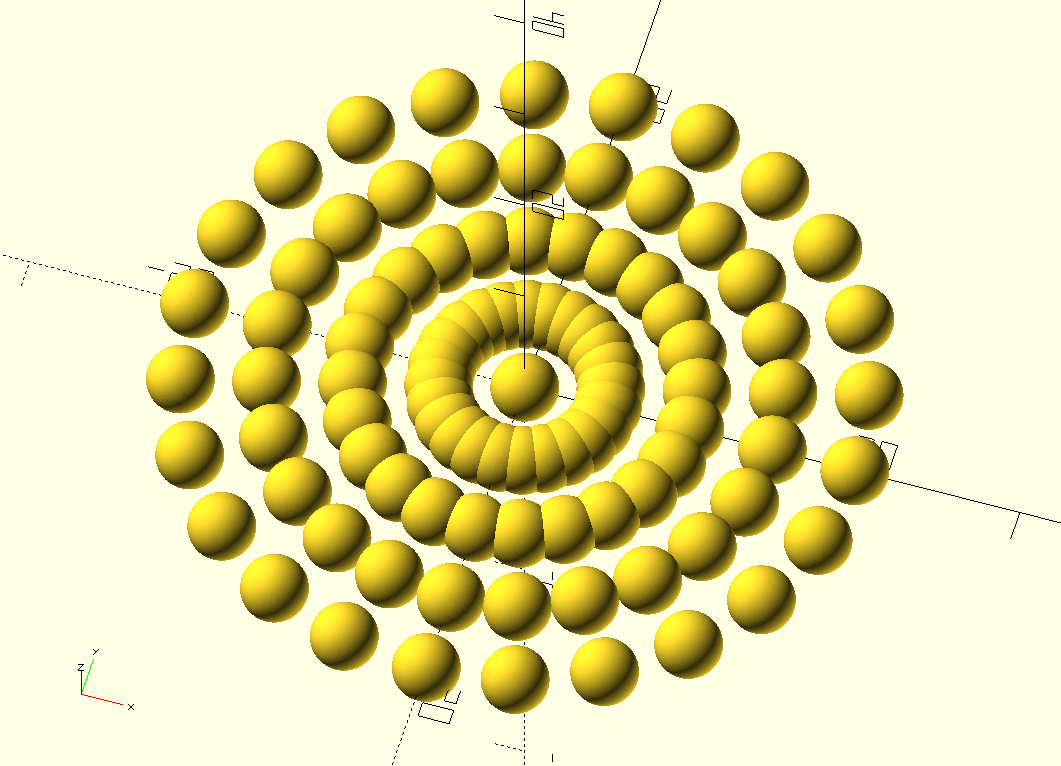
\includegraphics[width=\textwidth]{imagenes/anillos-de-esferas}
    \end{minipage}
    \caption{Solución de Cecilia para producir anillos de esferas.}
    \label{fig:anillos-de-esferas-cecilia}
  \end{figure}


  ---¡Vaamooss! ---exclamó Cecilia con aire triunfal, y alzando los
  brazos mientras contemplaba su solución en la figura
  \ref{fig:anillos-de-esferas-cecilia}. Comprobó con alegría que su
  sospecha funcionó: las líneas 4 a 7 de su texto creaban, como antes,
  un nuevo objeto (un anillo de esferas), y la línea 3 declaraba una
  nueva variable (\texttt{x}) que tomaba valores entre 20 y 0, a
  intervalos de 5 (el intervalo debía ser negativo porque \texttt{x}
  debía ir disminuyendo), con los cuales creaba anillos de distinto
  radio.

  Cecilia sintió que su mente comenzaba a poblarse de posibilidades
  innumerables y variadas, y que sus dedos no alcanzarían nunca a
  recorrerlas todas. <<Esto está buenísimo>> ---pensó.

  ---Te pido dos más, y terminamos por este capítulo ---pro\-me\-tió
  Antonia, cuya sonrisa delataba que compartía la misma alegría que
  Cecilia---. Hacé un cilindro de anillos de esferas, y un cono de la
  misma naturaleza. Te adelanto que este último es bastante más
  difícil...


  \begin{figure}[ht]
    \centering
    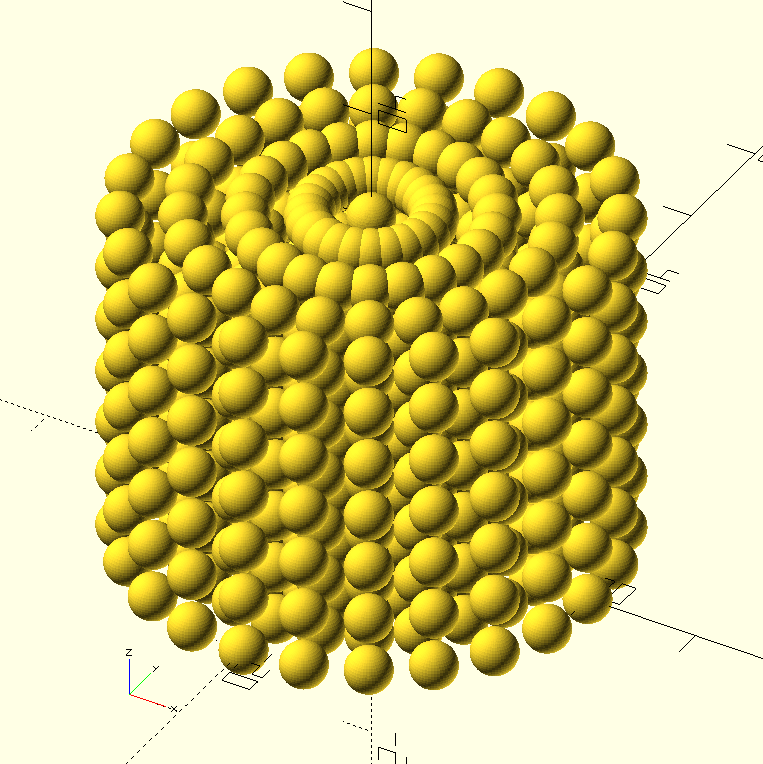
\includegraphics[width=.49\textwidth]{imagenes/cilindro-de-esferas}\hfill
    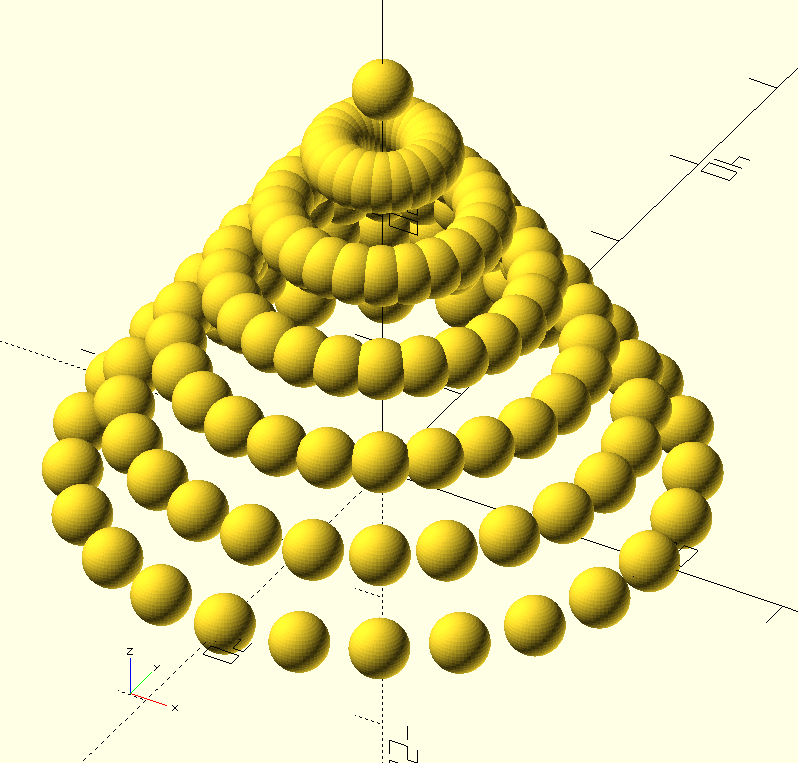
\includegraphics[width=.49\textwidth]{imagenes/cono-de-esferas}    
    \caption{Antonia propone a Cecilia escribir un cilindro y un cono
      de esferas.}
    \label{fig:cilindro-y-cono-de-esferas}
  \end{figure}


  A Cecilia le costó bastante el cono, aunque descubrió \mbox{---pa}\-ra su
  sorpresa--- que sólo requería el empleo de dos bucles, mientras que
  para el cilindro necesitó tres.

%\iftoggle{libro}{}{\vfill}

\section{Cilindro de esferas: una solución}


El cilindro no le resultó demasiado difícil a Cecilia; comprendió que
no se trataba de otra cosa que una repetición a lo largo del eje
\coord{Z} del anillo que ya había conquistado. Eso le sugirió el
empleo de un bucle más.


  \begin{figure}[ht]
  \begin{minipage}[]{.5\textwidth}
    \begin{lstlisting}
$fn=200;

for(z=[0:5:30])
 for(x=[20:-5:0])
  for(alfa=[0:15:359])
   rotate([0,0,alfa])
    translate([x,0,z])
     sphere(r=2);
    \end{lstlisting}%$
  \end{minipage}\hfill
    \begin{minipage}[]{.5\textwidth}
      \centering
      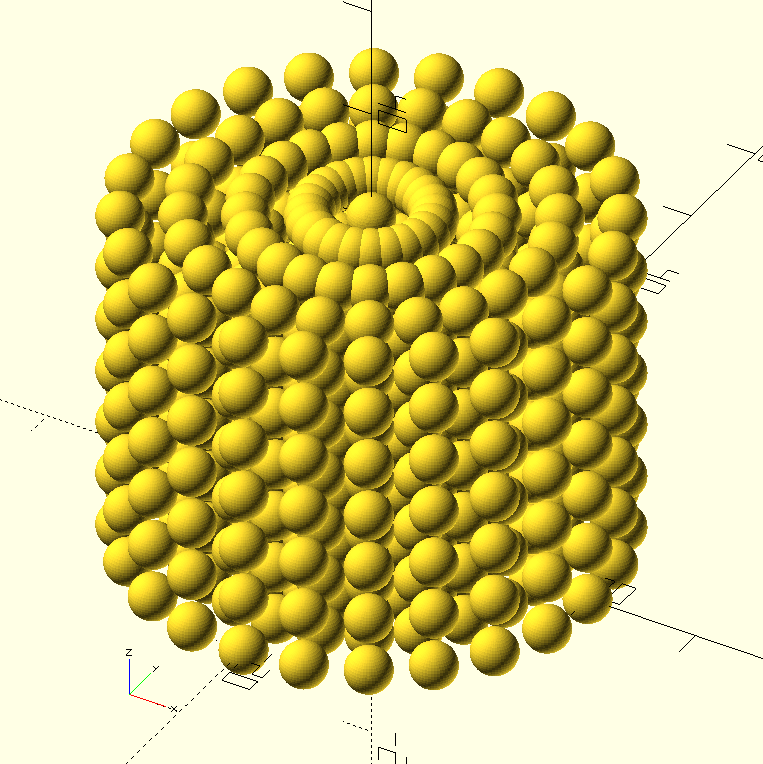
\includegraphics[width=\textwidth]{imagenes/cilindro-de-esferas}
    \end{minipage}
    \caption{Solución de Cecilia al cilindro de esferas.}
    \label{fig:cilindro-de-esferas}
  \end{figure}


  Las líneas 4 a 8 de la figura \ref{fig:cilindro-de-esferas} eran una
  mera copia de las que utilizó para escribir el anillo en la sección
  anterior, con una salvedad: en la línea 7, el `0' que indicaba la
  traslación en el eje \coord{Z} fue reemplazado por la variable
  `\texttt{z}', cuyo valor es determinado por el bucle de la línea 3:
  en él, se la hacía recorrer los valores de 0 a 30, en intervalos de
  a 5, creando de esa manera siete pisos de anillos.

\section{Cono de esferas: una solución}
  

El cono representó un verdadero desafío: Cecilia comprendió que no
sólo debía crear anillos de altura creciente, sino de radio
decreciente. Sin embargo, tras pensarlo un rato se convenció de que la
altura de cada anillo ($z$, digamos) y su correspondiente radio ($x$,
¿por qué no?) no eran independientes: a la altura máxima
($z_{\text{máx}}$, ¿soy original?) le correspondía el radio mínimo (de
hecho, un radio nulo), mientras que a la altura mínima (también de
valor nulo, al yacer en el plano \coord{XY}) le correspondía el radio
máximo ($x_{\text{máx}}$, ya que estamos). Evocando sus recuerdos de
Álgebra\footnote{El lector interesado y armado con la noción
  matemática de función puede deducirla sin más que considerar una
  relación lineal vinculando ambos valores.}  llegó a una relación
satisfactoria entre los valores de $x$ y $z$:
  \[x = x_{\text{máx}} - z \cdot \left( \frac{x_{\text{máx}}}{z_{\text{máx}}} \right) \]
  \begin{figure}[ht]
  \begin{minipage}[]{.5\textwidth}
    \begin{lstlisting}
$fn=200;
for(z=[0:5:30]) {
 x=20-z*20/30;
 for (alfa=[0:15:359]) 
  rotate([0,0,alfa])
   translate([x,0,z])
    sphere(r=2);
 }
    \end{lstlisting}%$
  \end{minipage}\hfill
    \begin{minipage}[]{.5\textwidth}
      \centering
      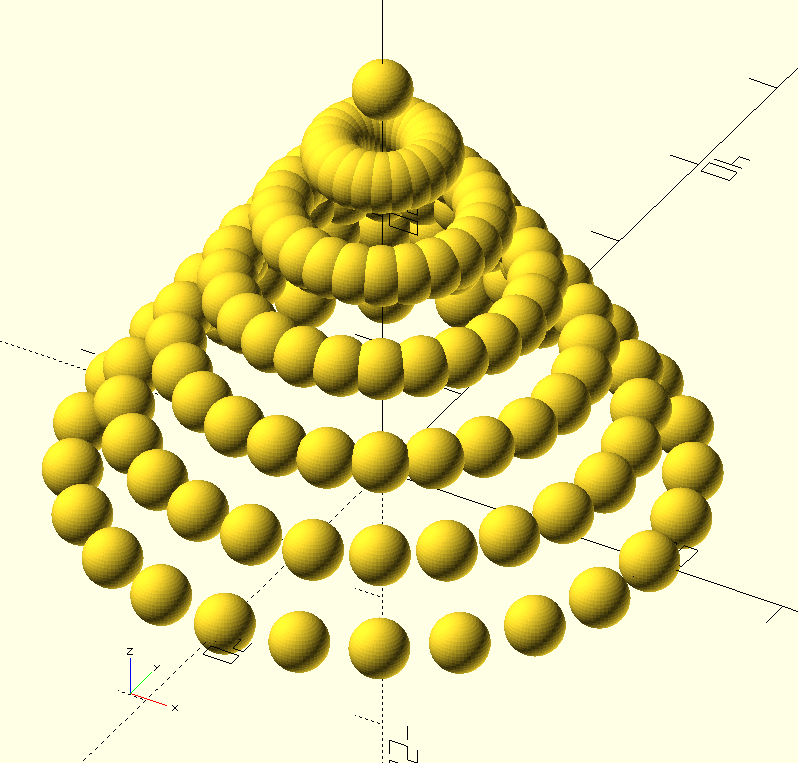
\includegraphics[width=.75\textwidth]{imagenes/cono-de-esferas}
    \end{minipage}
    \caption{Solución de Cecilia al cono de esferas.}
    \label{fig:cono-de-esferas}
  \end{figure}


  En primer lugar, entonces, declaró en la línea 3 el bucle que hace
  que \textbf{\texttt{z}} recorra las alturas de cada piso. Con ese
  valor, calculaba entonces en la línea 4 el correspondiente radio
  \texttt{\textbf{x}} del mismo. Y con ambos valores, creaba el debido
  anillo en las líneas 5 a 8. Las llaves de las líneas 3 y 9
  resultaban necesarios, puesto que el bucle de la línea 3 abarcaba
  más de una instrucción.


  
%%% Local Variables:
%%% mode: latex
%%% TeX-master: "../libro"
%%% End:
